\chapter{Specific Requirements}
\label{cha:requirements}

\section{External Interface Requirements}
\subsection{User interfaces}
The User Interface in every implementation should be intuitive and give the user the perception of control across the functionalities given from the application. The application has to support multiple languages, with a centralized label manager. This should be enforced by the coherence of all the functionalities across every the platform. Besides that, every platform must have a User Interface compliant with the latest major commercial standards available:
\begin{itemize}
\item Mobile
\begin{itemize}
\item The application will be developed with Xamarin.Forms and so the UI will be shared across the iOS and Android implementations. On top of that, the 2 versions must follow the iOS Human Interface Guidelines and the Android Material Design Guidelines.
\item Due to the huge variety of the Android devices, the application will provide the pixel perfect compliance relying on the 2 major screen sizes (normal, large) and 4 different densities (ldpi, mdpi, hdpi, xhdpi) depending on Android OS to auto-scale the missing ones.
\end{itemize}

\item Web
\begin{itemize}
\item The web application must be compliant with the W3C standards, concerning HTML and CSS. The UI should be modular and independent from business logic, supporting the major browsers (IE, Edge, Chrome, Firefox, and Safari).
\end{itemize}
\end{itemize}

\subsection{Hardware interfaces}
The application will require the authorization to access the user’s location, available through the GPS and/or the WiFi/Data connection. 

\subsection{Software interfaces}
The clients will implement the core functionalities interfacing with the Google Maps Distance Matrix API, Yahoo Weather and whenever possible the API exposed by the shared transport systems chosen by the user. 
Saving user's data will be managed through SQLite, with built-in hooks to encrypt them.

\subsection{Communication interfaces}
The application will be based on a service integration layer built upon REST API allowing all the different implementation to retrieve consistent information. 
This will allow the platform to ensure the scalability of the number of user and new features.

\section{Functional Requirements}
\label{sec:func_req}
The following are the functional requirements of the software, extracted from our analysis, concerning each actors of the system. Each of them consists of some scenarios and related use case, sequential and statechart diagrams.

\subsection*{User Login and Registration}
\subsubsection{Purpose}
Any user is encouraged to subscribe through the web application or the mobile one. The system provides the user the possibility to become a registered user by filling a registration form or directly accessing through third-party accounts like Google or Twitter. After authenticating, functionalities concerning the account management are also provided, so the user can easily:
\begin{enumerate}
	\item Login into his/her account.
    \item Recover forgotten password by resetting it
    \item Update account data.
\end{enumerate}
Users are simply asked to insert this information:
\begin{itemize}
	\item E-mail address
	\item Username
	\item Password
    \item Name
    \item Surname
\end{itemize}
Credentials are encrypted stored in the device so that the user must never insert them but the first time. Whilst asking for registration and logging in to access the application can be seen as a waste of time, it is designed for allowing the user to manage his/her own reminders and events both from the mobile and the web application and they are always synchronized.
\subsubsection{Scenario 1}
Alice decides to give the application a try, so, after downloading and launching it, she is displayed a login page where she is asked to sign up in order to access to all its services. She immediately notices the Google logo and, to avoid wasting time by creating another account, she decides to sign up with Google. Everything goes well, and she is welcomed by the user-friendly interface and the application is now fully working.
\subsubsection{Scenario 2}
Bob accesses Travlendar+ application through the web page and clicks on the \textit{Login} button. He is asked to enter his username and password, but figures out that he had never joined to the service before, so he goes back and decides to sign up. Being completely new, he creates a totally new account. When filling the form, he inputs \textit{Bob} as username. Turns out that this username has already been used so Bob is warned that that username is unavailable. He changes username, continues fulfilling the form and eventually, a window welcomes him by starting a little demo which guides him around the website. He is also informed that to fully access the application he must confirm the evidence of the registration by clicking the link sent via email.
\subsubsection{Use case}

\begin{table}[H]
\begin{center}
\begin{tabular}{|c||p{0.6\textwidth}|}
	\hline
    Name & Login \\ \hline
    Goal & G1 \\ \hline
    Actors & Registered User \\ \hline
    Assumptions & \begin{itemize}
    					\item The user has already signed up into the system. 
                        \item The user is not logged into the system yet.
                  \end{itemize} \\ \hline
    Events flow & \begin{enumerate}
                   		\item The user opens the \textit{login page} of the system;
                        \item The user types in username and password.
                        \item The system recognizes the identity and ensures that the user who is logging it is who he claims to be.
                        \item The user can visualize his personal calendar and access to the system's functionalities provided to him.
                     \end{enumerate} \\ \hline
   Exit conditions & The user is now logged into the system. \\ \hline
   Exceptions & The \textit{username and password} inserted are wrong, an error message is shown. The user is not logged.\\ \hline
\end{tabular}
\end{center}
\caption{Use case for user login.}
\label{usecase-login}
\end{table}

\begin{table}[H]
\begin{center}
\begin{tabular}{| l | p{0.6\textwidth} |}
\hline
Name & Registration \\ \hline
Actor & Unregistered user \\ \hline
Goal & G0 \\ \hline
Input condition & The user creates a new user account or signs up with third-party accounts. \\ \hline
Events flow & \begin{enumerate}
	\item The user decides whether he/she wants to create a completely new account or to undergo an application-based enrollment.
	\item Either the user is redirected to the third-party sign-up page and asked to insert his/her credentials or a registration form is loaded and the user is asked to compile it.\label{load-registration}
	\item In both cases, the user is asked to authorize the privacy policy and terms of conditions.
	\item If the user decided to create a new account, then he/she can confirm the registration by accepting the linked sent via email. No two-factor authentication is called for.
	\end{enumerate}
\\
\hline
Output condition & The system welcomes the user by informing him/her that the registration was done successfully. \\
\hline

Exception &  \begin{itemize}
	\item If username or similar data are already been taken or invalid username is provided, the user is warned to choose for a different username.
   	\item If no account exists when signing up through third-party services, they will also handle resulting possible errors.
	\end{itemize}
 \\ \hline
\end{tabular}
\end{center}
\caption{Use case for user registration.}
\label{usecase-registration}
\end{table}

\begin{figure}[H]
	\centering
	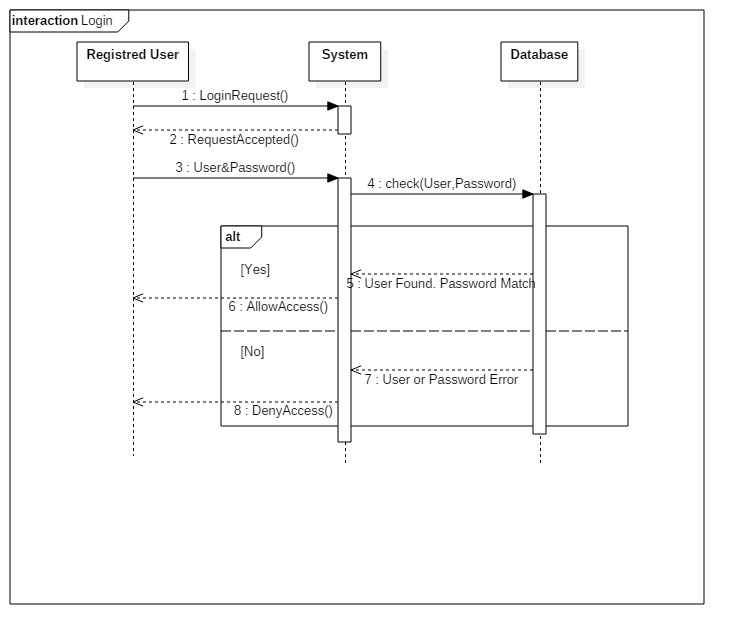
\includegraphics[width=6in]{./diagrams/SequenceLogin.png}
	\caption{Sequence Diagram: Login}
	\label{fig:SequenceLogin}
\end{figure}

\subsection*{Appointments overview and creation}
\subsubsection{Purpose}
The user of the application who has correctly logged in the web application or the mobile one, can view and organize the appointments into his own calendar. The system provides the user the possibility to see, create, modify or delete any appointments that he/she has inserted. In particular, the main features are as follows:
\begin{itemize}
\item View appointments: the user is given the possibility to view all the appointments, both with the general overview in the form of a grid, and the list view with appointments and the public means interleaved.
\item Create appointment: the user has to click on the specific date where he wants to add the new appointments and inserts the information below:
        \begin{enumerate}
        \item Name of appointment;
        \item Start time;
        \item End time;
        \item Recurrence (optional);
        \item Means of transport.
        \end{enumerate}
\item Modify appointment: the user simply clicks on the appointments that he has created so that he is able to update the information.
\item Delete appointment: the user through the same gesture of \textit{Modify appointment} can easily delete the appointment by clicking on the specific button.
\end{itemize}

\subsubsection{Scenario 1}
Alice, a young business consultant, plans all her appointments through the Travlendar+ application. Every Wednesday, the company decides to organize a refresher course. For this reason, she needs to add this appointment to her calendar.
Alice through the calendar interface, clicks on the first day course and adds the necessary information to create the appointment by using the form: event name, start time, end time, recurrence, means of transport. The system checks that the new appointment meets each requirement and asks Alice to confirm. Once confirmed, the event is displayed in her list of appointments. Unfortunately, the company after a few days, deletes the refresher course, so Alice wants to delete the appointment from her calendar. Alice easily accesses the event and modifies it. By clicking the corresponding button, she deletes the event and all the saved recurrences. The system asks Alice if she is really sure to perform the operation, she confirms and the event is deleted from the calendar.

\subsubsection{Scenario 2}
Bob, after correctly signing up to Travlendar+, decides to check the appointments of the day through the calendar. While he’s scrolling the appointment list, he notices that one of the places of meeting was entered incorrectly. By simply clicking on the event, Bob is able to update the information. The system checks that the updated appointment meets each requirement. After calculating the time needed to reach the place of the appointment, the system warns Bob that the travel time between the previous and the updated event is not enough to reach the place of the appointment. However, the system asks Bob if he wants to confirm or update the event. He doesn’t choose to update the event, so changes are not made. Bob accesses the event and modifies it again, but in this case, he deletes the event by clicking on the specific button. The system requires confirmation and the event is deleted form the calendar.

\subsubsection{Use case}
The use case for creating an appointment is shown in Table \ref{usecase_app}.

\begin{table}
\centering
	\begin{tabular}{|c||p{0.6\textwidth}|}
		\hline
		Name & Create appointment \\ \hline
		Actors & User \\ \hline
		Assumption & The user needs to insert a new appointment in his/her personal calendar \\ \hline
		Pre-Conditions & \begin{itemize}
			\item The user has successfully signed to the system.
			\item The user has already opened the window with the insertion form.
		\end{itemize} \\ \hline
		Flow of events & \begin{enumerate}
			\item The user creates a new appointment by inserting all the information needed in order to adding a new event correctly in his own calendar.
			\item The system checks if the appointment inserted can be successfully validated. This means that simple checks against the time (the start one should be less than the end one) and the date (should not be an expired date) are done. \textit{Note:} overlapping events check is done at a second stage. 
			\item The user is informed by a warning message about the actual validation of the appointment.
			\item The user have to confirm o reject the insertion of the appointment.
		\end{enumerate} \\ \hline
		Post-Conditions & The appointment of the user has been stored into the system in the event that he has confirmed the inclusion. \\ \hline
		Exception & An internal system error makes impossible to store the reservation data. The user is notified of the error \\ \hline		
	\end{tabular}
\caption{Use case for create appointment.}
\label{usecase_app}
\end{table}
    
\subsubsection{Sequence diagram}
The sequence diagram for creating an appointment is illustrated in Figure \ref{fig:SequenceLogin}.
\begin{figure}
	\centering
	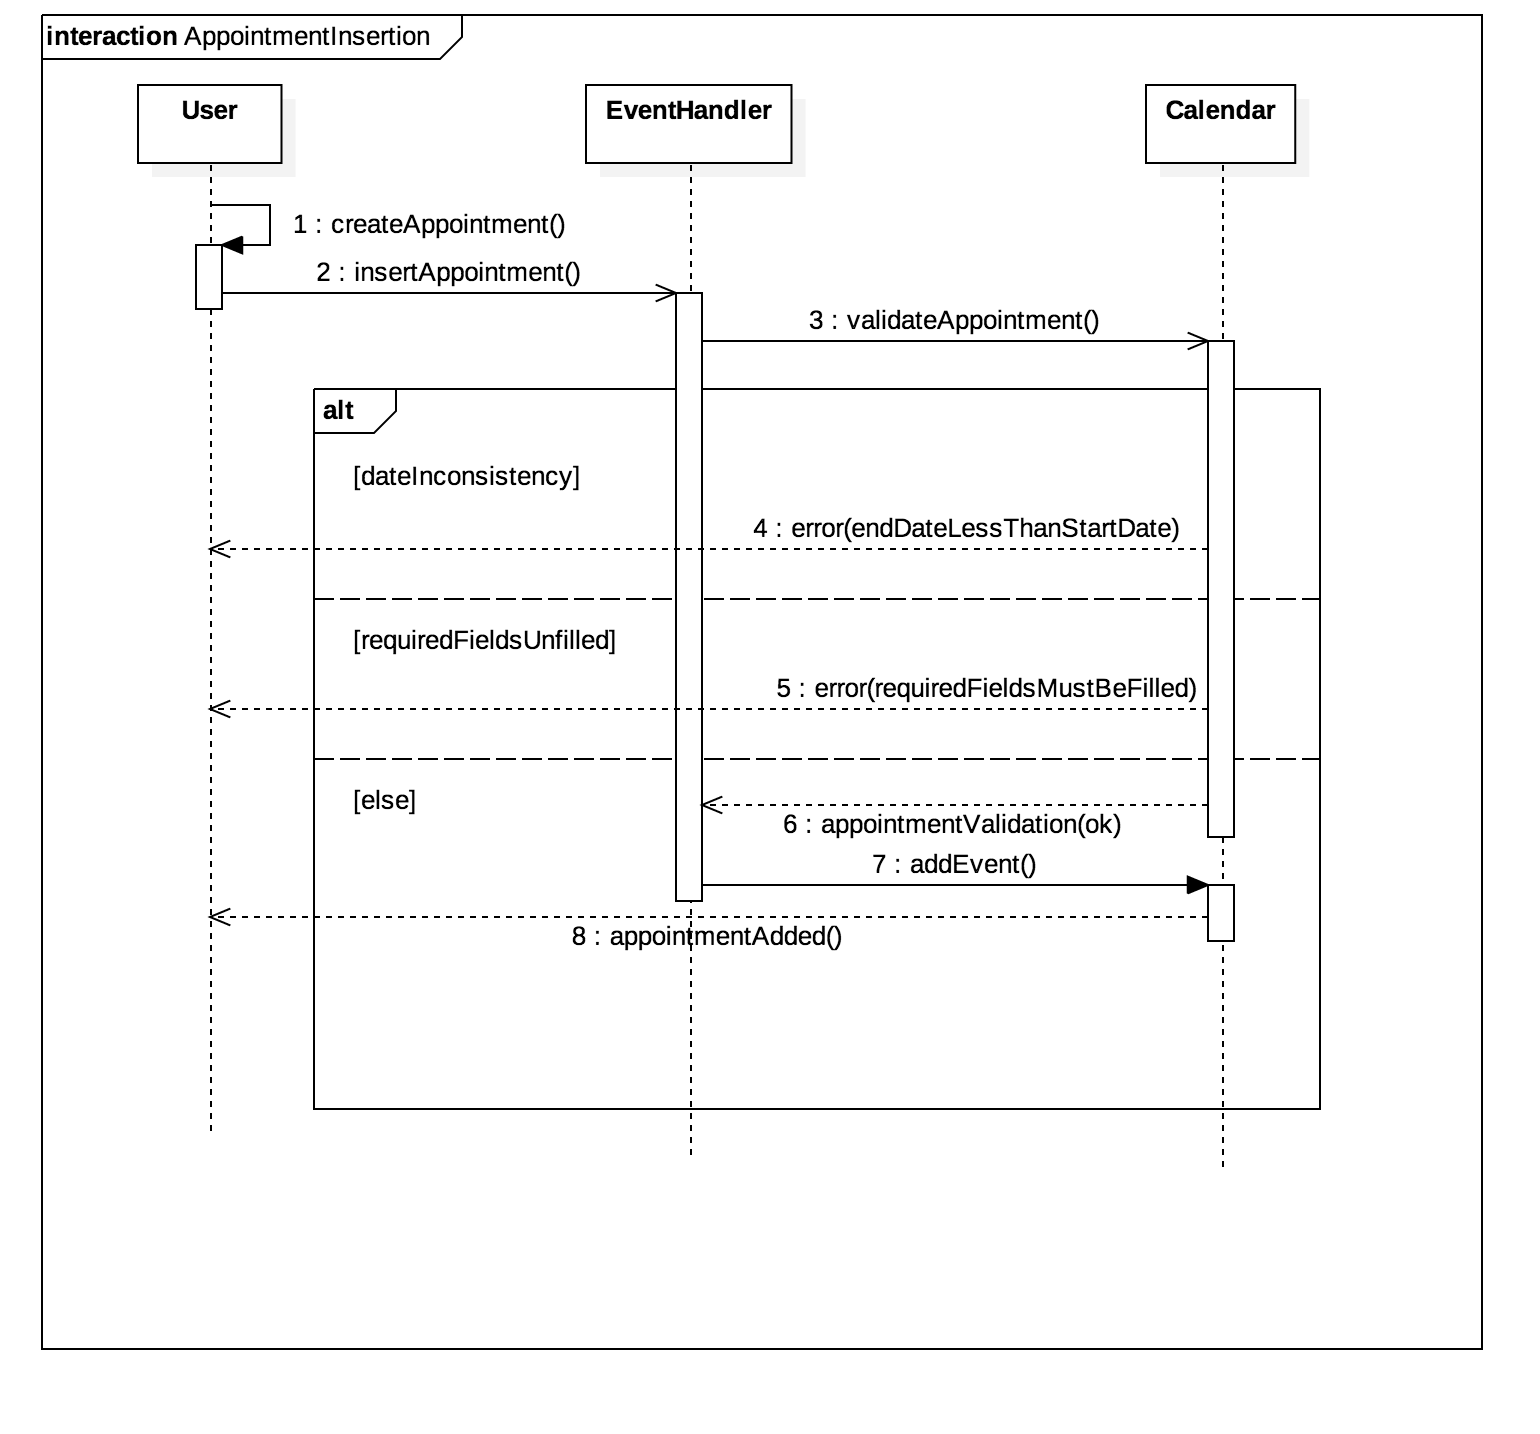
\includegraphics[width=6in]{./diagrams/AppointmentInsertion.png}
	\caption{Sequence Diagram: Create Appointment}
	\label{fig:SequenceAddApp}
\end{figure}

\subsubsection{Mockup}
The mockup of the appointments overview and the list view are shown in Figure \ref{fig:MockupAppointments} and in Figure \ref{fig:MockupListing}, the menu of the application is shown in Figure \ref{fig:MockupMenuView} and the creation of appointments is shown in Figure \ref{fig:AppointmentCreationMockup}.
\begin{figure}
	\centering
	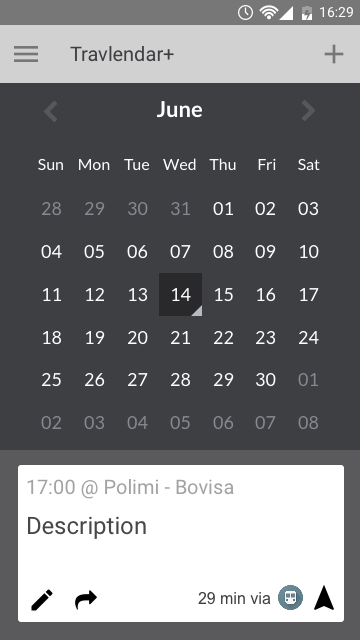
\includegraphics[width=4.5in]{./images/home.png}
	\caption{Overview appointments mockup.}
	\label{fig:MockupAppointments}
\end{figure}
\begin{figure}
	\centering
	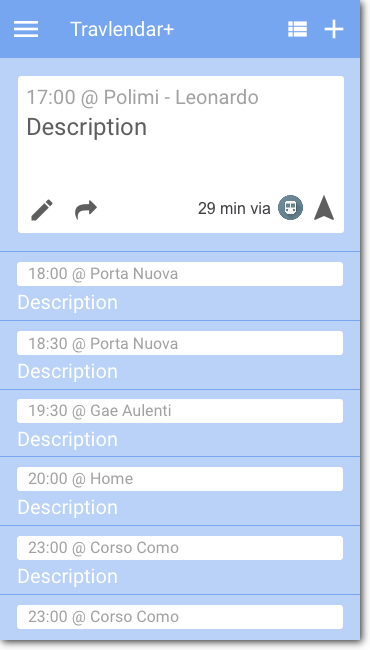
\includegraphics[width=4.5in]{./images/listing.png}
	\caption{Listing view appointments mockup.}
	\label{fig:MockupListing}
\end{figure}
\begin{figure}
	\centering
	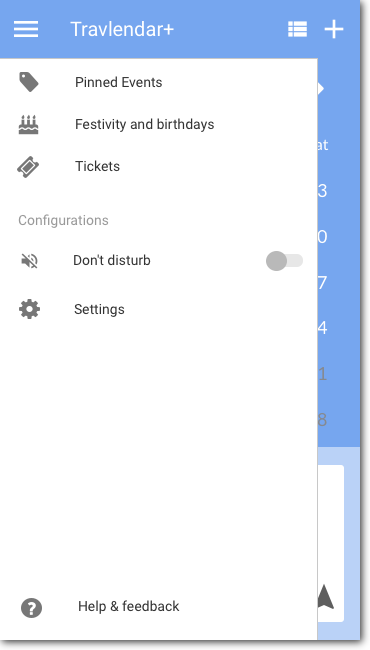
\includegraphics[width=4.5in]{./images/menu.png}
	\caption{Menu view mockup.}
	\label{fig:MockupMenuView}
\end{figure}
\begin{figure}
	\centering
	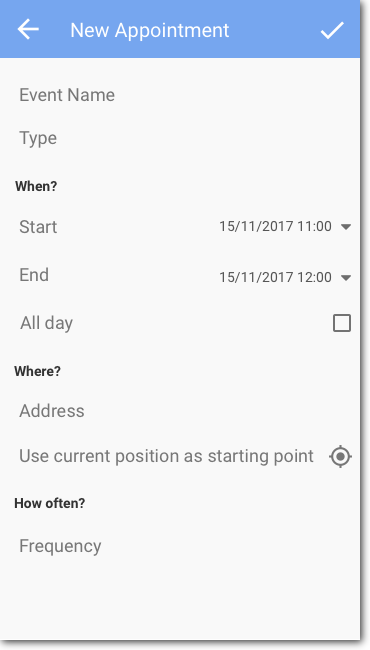
\includegraphics[width=4.5in]{./images/appointment.png}
	\caption{Creation appointment mockup.}
	\label{fig:AppointmentCreationMockup}
\end{figure}

\subsection*{Time and route travel}
\subsubsection{Purpose}
A user who successfully creates events may wish to take advantage of one of the most interesting feature of Travlendar+, which concerns both time and itinerary. This makes Travlendar+ an enhanced calendar-based application. Particularly, a user can add as many events as he/she may want, and the system will be responsible to arrange time slots so as to ensure that he/she is never going to be late. The system allows the user to insert the location of the event as well so as to instruct him to take the best itinerary to reach such location. To compute the best route in terms of both space and time a sequence of calculations will be executed. Various factors - both that can be handled by the user and that which cannot - are considered.

\subsubsection{Scenario 1}
Alice is a manager who needs to go often around the city for work to meet customers. Since living in a big city and having to wake up soon, she knows that in the peak hours it's difficult to move around the city, and the system is aware of this too. She often needs to move around the entire city pretty fast. So, whenever she wants to see the task ahead, she knows she is in good hands, in fact the system typically proposes her the best route which consists of taking the bus or the underground train, or - often - a combination of them so that she can avoid the traffic of the city. 
\subsubsection{Scenario 2}
Charlie, who is a little bit messy and unmindful, inserts multiple appointments for work for the current day and fills up the entire time window for which lunch is supposed to be done. Fortunately, the application reminds here not to forget to have lunch so he is prompted with a dialog to choose when he would like to insert lunchtime. Then he adds two appointments which are too close together. Itinerary is calculated anyway, but no feasible route is possible to reach the destination. The system however recognizes that 5 minutes before the end of the first appointment a bus will pass by there, so he is informed that if he desires to be in time to the upcoming event he will just have to confirm system's proposal. He accepts and a remainder for leaving earlier the first appointment is automatically set. 
\subsubsection{Scenario 3}
Bob promotes conferences to sensitize environmental sustainability issues. Whenever he is invited to give lectures, he always tries to opt for travel means whose environmental impact is as low as possible in order to minimize, among other things, the carbon footprint. So he started using Travlendar+ because he is aware of this unique functionality which suggests convenient travel means for reaching various locations. Being the ecological option enabled, the system advises Bob to avoid means like cars and taxis, and, depending on how far away the destination is, the system will tell him to go on foot, or will locate the nearest bike sharing system or, at most, to use urban transports.
\subsubsection{Scenario 4}
Eve, a young girl of regular habits, who has seen an advertising of the application online, has started using it recently. At the first use, a welcome message and a little demo are shown and she is moved into another window where she is asked to set some preferences in order to fully customize the application. When checking the age, the system recognizes that she is a minor, so car driving and car sharing are disabled by default. The system understands that she's accustomed to inserting recurring events like going to school, so she is notified in advance if there's some traffic which may require here to leave home earlier. What's more, the system realizes that most places are reached walking - regardless of the fact that it is not that near or not - and, after a while, the system displays possible paths that can be taken on foot by default.

\subsubsection{Use case}
The use case for the travel time arrangement is shown in Table \ref{usecase_traveltime}, whereas the use case for the travel route handling is shown in Table \ref{usecase_travel_location}.
\begin{table}
\centering
	\begin{tabular}{|c||p{0.6\textwidth}|}
		\hline
		Name & Travel time arrangement \\ \hline
		Actors & System manager \\ \hline
		Input condition & The user has already added at least one appointment and has been validated. \\ \hline
		Flow of events & \begin{enumerate}
			\item The user may want to create further appointments.
			\item The system figures out the time window between one event and another, which means that attempts to compute whether there's enough time to get to the next appointment successfully, which is supposedly - but not necessarily - to be in a different location.
			\item The system warns the user if a scheduled appointment is too adjacent to another or cannot be easily reached.
			\item The system checks and rejects two appointments overlapping with each other (whose start date and time, and end date  and time are identical).
            \item The system ensures that at least an half an hour - at the discretion of the user to change slotted time - is reserved for lunchtime.
		\end{enumerate} \\ \hline
		Output condition & The user can trust the system that all his/her appointments are properly organized. \\ \hline
		Exception & There's no particular exception which may occur. A user, due to unforeseen circumstances, may not respect some appointments. This cannot be obviously handled by the system and no warnings are displayed.  \\ \hline		
	\end{tabular}
\caption{Use case for travel time arrangement}
\label{usecase_traveltime}
\end{table}

\begin{table}
\centering
	\begin{tabular}{|c||p{0.6\textwidth}|}
		\hline
		Name & Travel route handling \\ \hline
		Actors & System manager \\ \hline
		Input condition & The user has already added at least one appointment and has been validated. \\ \hline
		Flow of events & \begin{enumerate}
			\item A check of the user preferences is performed the very first time or whenever local settings have been changed.
            \item The system controls date of event. If the event is scheduled for the current day it continues with calculating the path otherwise, otherwise it is not considered for now.
            \item The system asserts that the destination location of the newly added event exists and is reachable and attempts computing the best travel path to reach the location in time.
			\item The system performs specific checks against the weather condition, the fact that a bike sharing system is in the close proximity and whatnot.
            \item Some confirmation dialog asking if there's a preference for a particular itinerary or public mean may show up in case multiple reasonable routes are found.
            \item The system provides the user the best travel path with selected means of transport (or a combination of them) in accordance with user's preferences.
            \item The user is asked to confirm, choose for a different path and following recalculation or dismiss.
		\end{enumerate} \\ \hline
		Output condition & A suitable and reasonable travel path is guaranteed to be found. \\ \hline
		Exception & There's no particular exception.  \\ \hline		
	\end{tabular}
\caption{Use case for travel location arrangement}
\label{usecase_travel_location}
\end{table}

\subsubsection{Sequence diagram}
The sequence diagram of the handling of checks process carried out by the system is illustrated in Figure \ref{fig:TravelTime}.
\begin{figure}
	\centering
	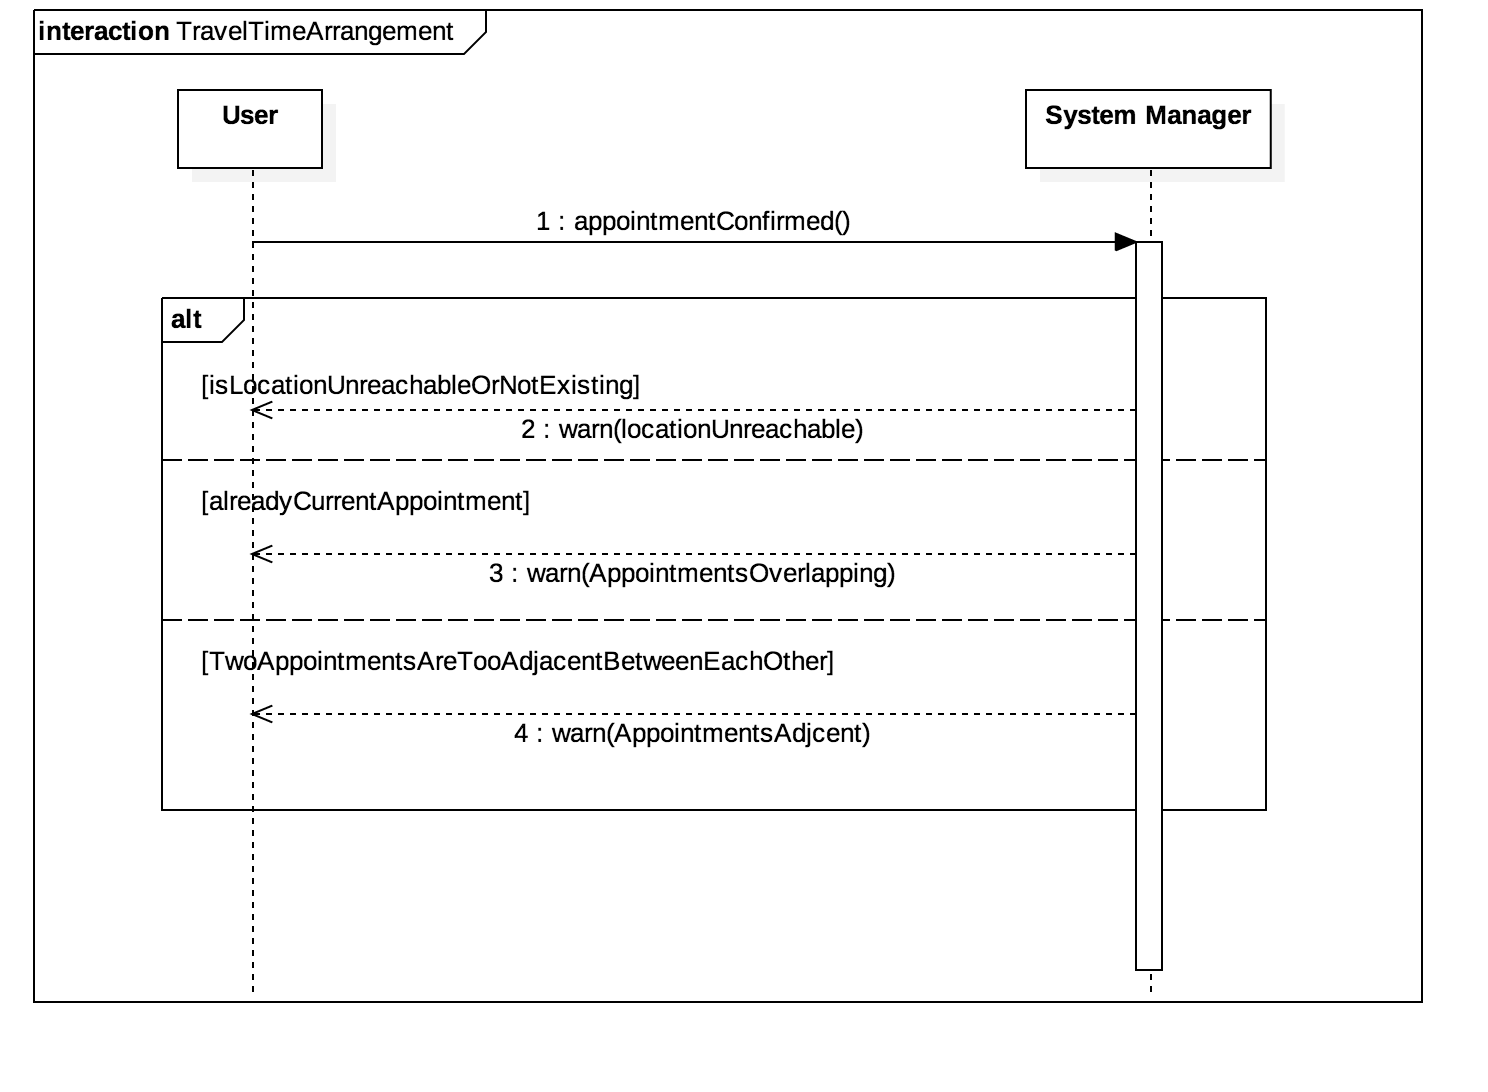
\includegraphics[width=6in]{./diagrams/TravelTimeArrangement.png}
	\caption{Sequence Diagram: Travel Time Arrangement.}
	\label{fig:TravelTime}
\end{figure}

\subsubsection{Statechart}
The statechart of the action undertaken by the system is illustrated in Figure \ref{fig:StateChecks}.
\begin{figure}
	\centering
	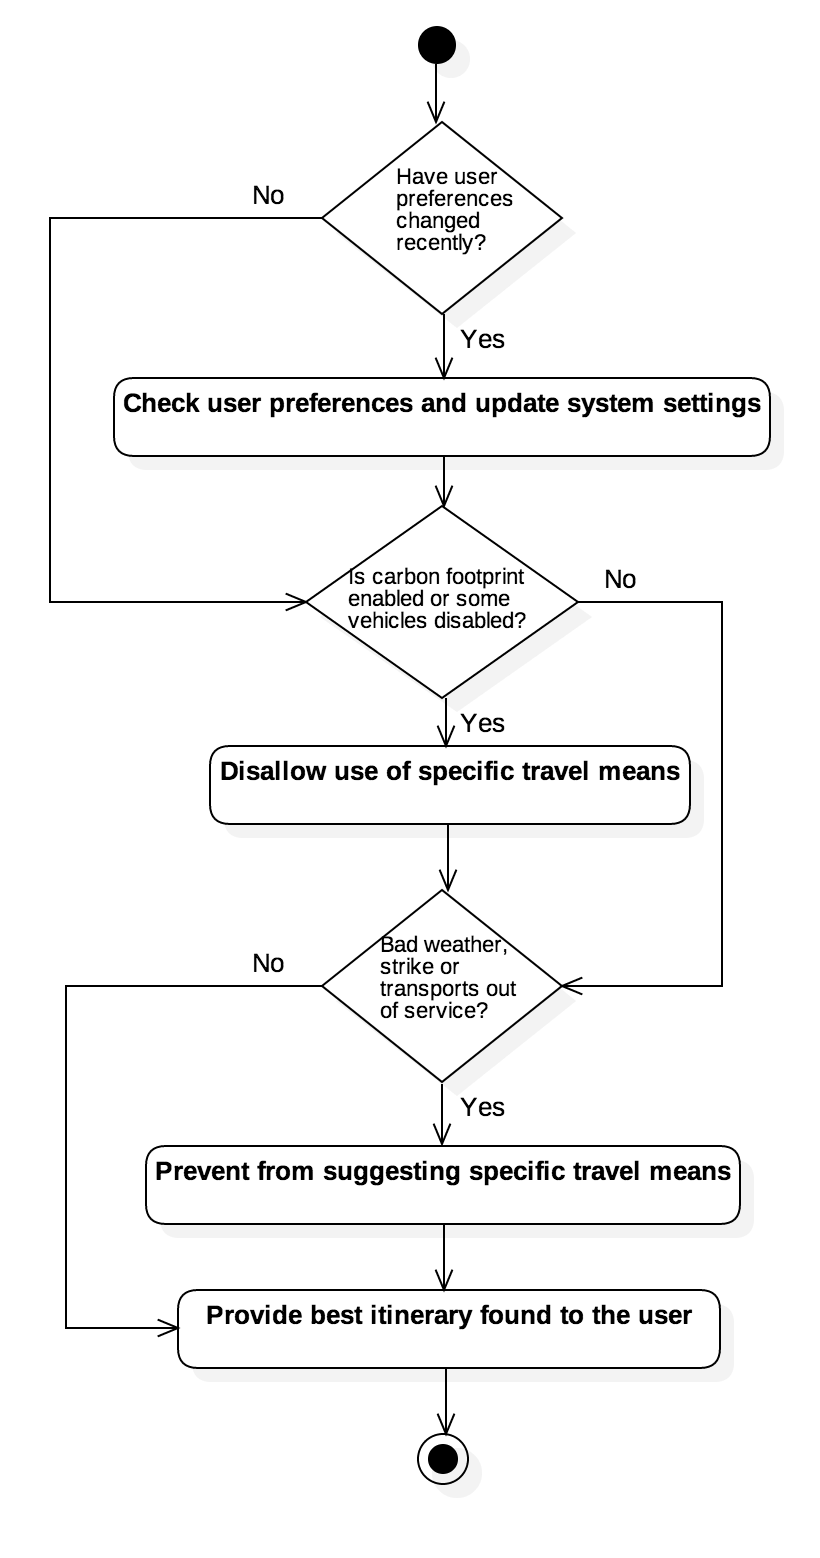
\includegraphics[width=5in]{./diagrams/StatechartChecks.png}
	\caption{Statechart: Travel Time Arrangement.}
	\label{fig:StateChecks}
\end{figure}

\subsubsection{Associated functional requirements}
\begin{enumerate}
\item The system will ask the user the first time to authorize the use geolocalization (estimation of the current position).
\item The system calculates the best itinerary only for events for the current day. Events for the following days, after being added to the calendar, are actually evaluated only when that specific day comes.
\item The system takes into account the current position as starting point by default.
\item The system allows the user to customize travel means to be taken according to his/her preferences.
\item The system computes the best route based on both user preferences and on factors which cannot be controlled by the user (belong to the external world).
\begin{itemize}
\item The system checks user preferences every time they have been changed.
\item The system disallows using car if the user is not 18-year-old yet.
\item The system will not provide a route with a specific transport, if the user has chosen not to use it.
\item The system will locate the nearest bike sharing system if the user is accustomed to riding a bike and favourable conditions occur.
\item The system will be likely to suggest walking instead of using motor vehicles if distance may take a little bit longer on foot but there's traffic jam.
\item The system will unlikely suggest walking if it is going to start raining.
\item The system will unlikely suggest car or taxis if the user has enabled carbon footprint optimization option.
\end{itemize}
\item The system will notify the user - when an event is approaching - that car can be taken if traffic is pretty much smooth, or underground train will be near there within few minutes, if the user is close to a station.
\item The system will reserve at least half an hour for lunchtime, or any other kind of breaks - if requested by the user.
\end{enumerate}

\subsubsection{Mockup}
The mockup of the itinerary resolved with navigation with car is shown in Figure \ref{fig:MockupMapCar}, whereas the itinerary with navigation with public transports is shown in Figure \ref{fig:MockupMapPt}. The mockup of settings preferences is shown in Figure \ref{fig:MockupSettings}. Finally, the mockup of notifications provided by the application is shown in Figure \ref{fig:MockupNotifications}.
\begin{figure}
	\centering
	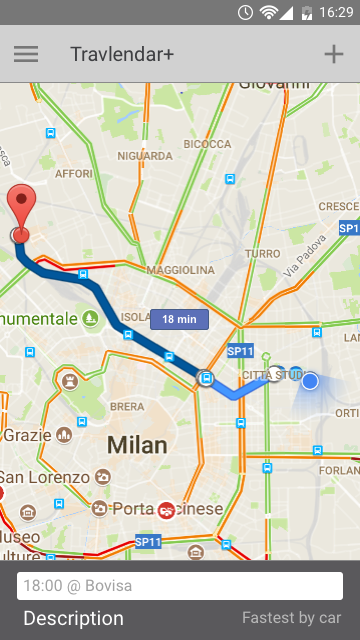
\includegraphics[width=4.5in]{./images/map_car.png}
	\caption{Navigation with car mockup.}
	\label{fig:MockupMapCar}
\end{figure}

\begin{figure}
	\centering
	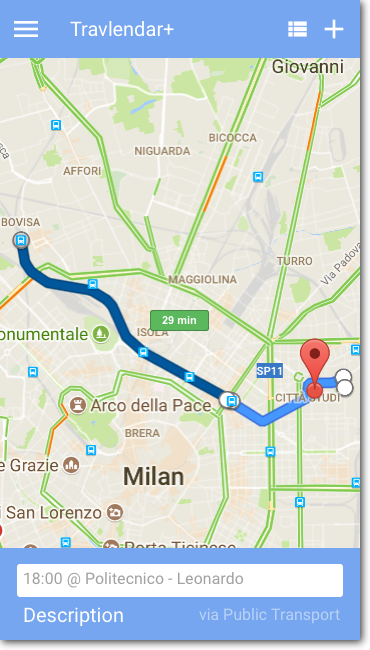
\includegraphics[width=4.5in]{./images/map_pt.png}
	\caption{Navigation with public transports mockup.}
	\label{fig:MockupMapPt}
\end{figure}

\begin{figure}
	\centering
	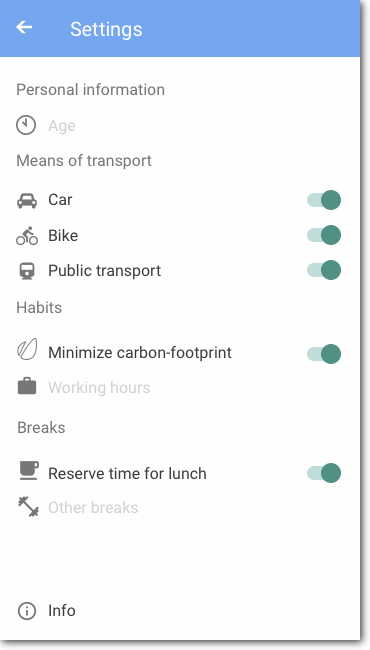
\includegraphics[width=4.5in]{./images/settings.png}
	\caption{User preferences settings mockup.}
	\label{fig:MockupSettings}
\end{figure}

\begin{figure}
	\centering
	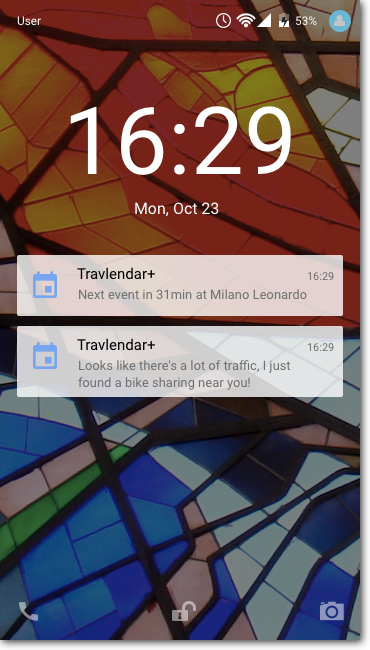
\includegraphics[width=4.5in]{./images/lockscreen.png}
	\caption{Application notification mockup.}
	\label{fig:MockupNotifications}
\end{figure}
\vspace*{26\baselineskip}

\subsection*{Purchase tickets and use rental service}
\subsubsection{Purpose}
One of the main feature of Travlendar+ is the possibility to display into the user's events schedule which kind of means of transport the user should take to reach the location of each appointments. Particularly, a user can take public transportation by buying tickets direct from the application or by inserting his pass code. If a user should take a taxi, he can easily book it by calling the local taxi service company. 
In addition, the application allows user the possibility to locate and take a shared transport of a vehicle sharing system like bike or car, simply from the application interface.

\subsubsection{Scenario 1}
\subsubsection{Scenario 2}
\subsubsection{Use case}
The use case diagram for mobility selection is shown in Figure \ref{fig:useCaseMobility}.
\begin{figure}
	\centering
	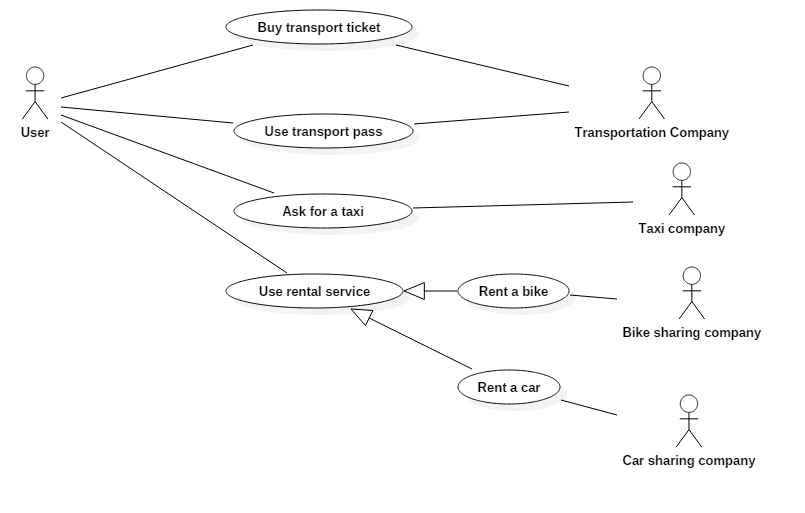
\includegraphics[width=6in]{./diagrams/TransportationUseCase.png}
	\caption{Use case diagram for mobility selection}
	\label{fig:useCaseMobility}
\end{figure}

\begin{table}
\centering
	\begin{tabular}{|c||p{0.6\textwidth}|}
    \hline
    Name & Purchase Tickets \\ \hline
    Actors & User \\  \hline
    Input condition & The user has already added at least one appointment and has been validated \\ \hline
    Flow of events & \begin{enumerate}
    \item The user may want to buy a public transport ticket
    \item The system forward the request to an external service in order to process the data and check the availability of the ticket.
    \item The external transport company API checks if there are tickets which 				are still purchased and asks to user the confirmation of buy the ticket.
    \end{enumerate} \\ \hline
     Output condition & The QR code of the tickets that he has purchased are added into the specific windows where the user can manage all his public transport ticket. \\ \hline
     Exception & The ticket may not be available for a specific means of transport (metro, bus, tram) \\ \hline
	\end{tabular}
\caption{Use case for purchase tickets}
\label{usecase_tickets}
\end{table}

\subsubsection{Sequence diagram}
The sequence diagram of the purchase tickets process is illustrated in Figure \ref{fig:useCaseMobility}.
\begin{figure}
	\centering
	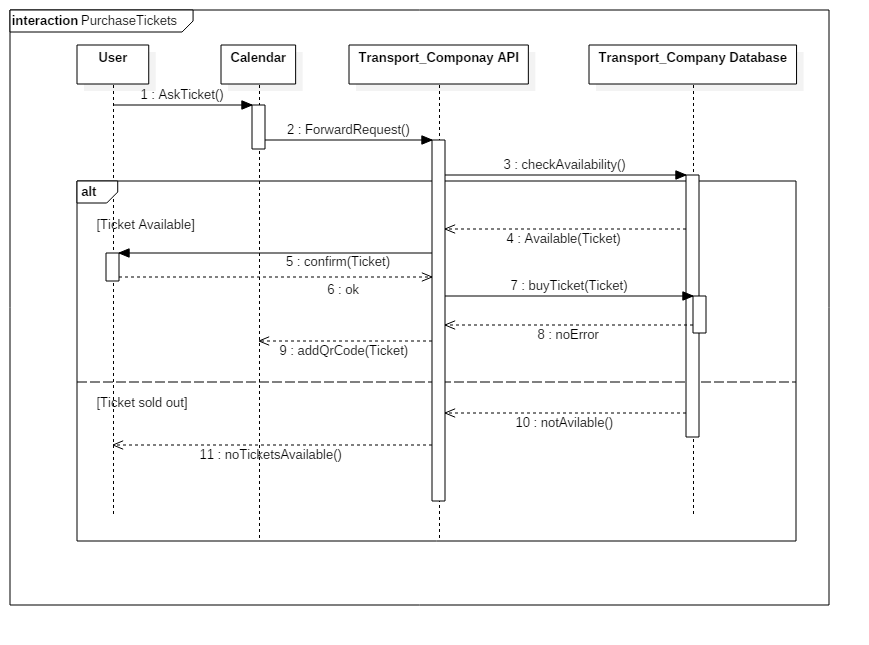
\includegraphics[width=6in]{./diagrams/PurchaseTickets.png}
	\caption{Sequence diagram: Purchase Tickets}
	\label{fig:useCaseMobility}
\end{figure}

\section{Performance Requirements}
\label{sec:perf_req}
The user experience across the application should be fluid and with zero waiting time moving between the sections. Besides, there are a number of requirements that implies third party information retrieved through asynchronous requests so, the previous requirement can allow some tolerance.

\begin{enumerate}
\item There is no limit to the number of users registered to the application.
\item There is no limit to the number of the simultaneous users of the application.
\item The login process must be completed in less than 5 seconds once submitted the data.
\item The date text fields have to validate dates in real time.
\item The application going back to foreground has to be in the same state as when it was going to background
\end{enumerate}

\section{Design Constraints}
\subsection{Standards compliance}
The application will be developed with the MVVM architectural pattern to allow the unification of the business logic and preserving the coherence across all the various implementations.
The implementation on iOS and Android will be compliant with the App Store Review guidelines and Android Compatibility Definition Document.
The web-app platform must be compliant with the W3C standards.

\subsection{Hardware limitations}
The application relies on the usage of the GPS location and Internet access. In any case of disabled GPS or energy-saver option that prevents the retrieval of the User’s location or in case of no connectivity the application will not provide the user the ETA or the route navigation to reach an event nor the login function if the user is logged out.

\subsection{Any other constraint}

\section{Software System Attributes}
\subsection{Reliability}
The application should have a 100\% uptime in each designed scenario. Since the application relies on different systems API’s there is room to accept small shifts in this requirement.

\subsection{Availability}
Concerning the mobile implementations the application will be available in the App Store and Play Store, rather, the desktop implementation will be available through the web app.
Eventually, there could be implementations of the project with Xamarin.Mac and UWP on Mac and Desktop available through the App Store and Microsoft Store.

\subsection{Security}
The applications will perform every request in HTTPS to preserve the security of the user. 
Data that have to be stored in the device, will be encrypted with third-party libraries to avoid leakage of the user’s information.

\subsection{Maintainability}
The implementations will be developed with the MVVM architectural pattern allowing a modular integration of future new features or changes in the requirements. 
The application will rely on Google Maps API in order to maintain its core functionalities and not on other third-party libraries that could be deprecated in future OS versions.

\subsection{Portability}
The clients are implemented with Xamarin giving support to OS’s 3 versions older than the last one available for each platform. (iOS 9-10-11, Android 6,7,8)
The applications will rely upon the MvvmCross framework to have the ecosystem needed to share the most code across the platforms.
The web-app will be based on AngularJS.
Our back-end service will be based on AWS Cognito Identity Services to allow scalability and integration with the business logic that is required. 
Changes from the normal workflow will be addressed with AWS Lambda or EC2 instances whenever needed.
